\subsection{Parallélisation des méthodes itératives}
La partie résolution de système linéaire creux représente souvent la partie qui consomme le plus de temps dans une simulation numérique, par exemple dans la simulation de réservoir cela peut représenter jusqu'à 80~\% du temps de simulation.
%
Il est donc essentiel de paralléliser cette partie du code.
%
Les noyaux de calcul les plus coûteux utilisés dans les méthodes itératives préconditionnées par une méthode ILU sont :
\begin{itemize}
  \item la factorisation ILU;
  \item les résolutions triangulaires;
  \item le produit matrice vecteur creux;
  \item le produit scalaire.
\end{itemize}
La parallélisation des méthodes de Krylov revient à paralléliser les noyaux de calcul cités précédemment.
%
L'une des méthodes de précondionnement parallèles les plus courantes est la méthode de Jacobi par blocs.
%
Dans cette méthode, nous découpons des blocs dans la matrice et nous appliquons notre préconditionneur sur chaque bloc.
%
Ces blocs proviennent d'un partitionnement du graphe d'adjacence (Fig.~\ref{fig:domain}) de la matrice à l'aide d'un logiciel de partitionnement, tel que Scotch ou Metis, avec pour objectif un bon équilibrage de charge.
%
La matrice est ensuite réordonnée pour que la numérotation des cellules à l'intérieur d'un domaine soit contiguë.
%
Ces domaines formeront des blocs dans la matrice sur lesquels nous appliquerons notre préconditionneur ILU.
%
Avec autant de blocs que de coeurs de calcul, nous pouvons factoriser tous les blocs parallèlement.
%
Cette méthode ignore donc les interactions inter-domaine et fournit donc un bon préconditionnement.
%
Sur la figure~\ref{fig:domain_jacobi}, les entrées de la matrice en dehors des blocs ne seront pas utilisées par la factorisation ILU ni par les résolutions triangulaires.
\begin{figure}[!h]
     \begin{center}
        \subfigure[Exemple d'une décomposition en quatre domaines.]{
          \label{fig:domain}
          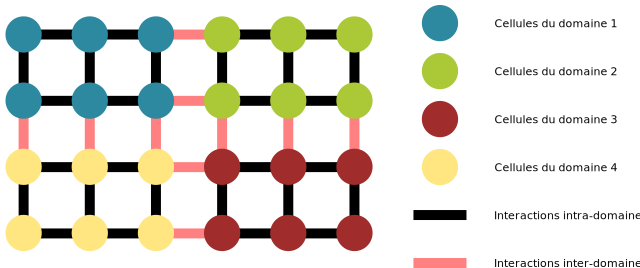
\includegraphics[width=\textwidth]{domain}
        }
        \subfigure[Une matrice ordonnée par domaine. Les entrées en dehors des blocs seront ignorées lors de la factorisation ILU.]{
          \label{fig:domain_jacobi}
          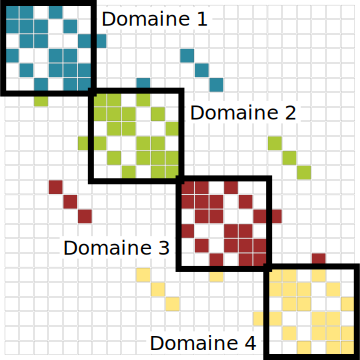
\includegraphics[width=0.50\textwidth]{domain_jacobi}
        }
    \end{center}
    \caption{Exemple d'une décomposition de domaine appliquée à une méthode de Jacobi par blocs.}
    \label{fig:jacobi}
\end{figure}
Les deux autres noyaux de calcul (le produit matrice vecteur creux et le produit scalaire) peuvent être parallélisés facilement.
%
Dans le cas du produit matrice vecteur creux, chaque coeur de calcul s'occupera de multiplier un ensemble de lignes de la matrice.
%
Cet ensemble peut provenir de la décomposition de domaine faite pour la méthode Jacobi par bloc, mais ce n'est pas obligatoire.
%
Pour le produit scalaire, chaque coeur de calcul s'occupera de multiplier un ensemble d'éléments des deux vecteurs.

La méthode de Jacobi par blocs n'affecte donc que la partie préconditionneur des méthodes itératives.
%
Le nombre de blocs aura un impact sur la convergence de la méthode itérative utilisée,
%
Cet impact n'est pas facilement prédictible et dépendra du problème étudié.
%
Il est donc quasiment impossible de connaître le nombre de blocs optimal nécessaire pour avoir un bon rapport parallélisme sur nombre d'itérations.
%
C'est pourquoi nous allons essayer de réduire au minimum le nombre de blocs pour toujours obtenir les meilleures performances.
%
Pour cela, nous allons devoir utiliser une autre forme de parallélisme qui s'appliquera à l'intérieur d'un bloc.
%
Nous aurons donc du parallélisme sur deux niveaux :
\begin{itemize}
  \item sur les blocs de la matrice avec la méthode Jacobi par bloc;
  \item à l'intérieur des blocs en parallélisant la factorisation ILU.
\end{itemize}
%
Notre but étant d'affecter le moins possible la qualité du préconditionneur.
